%%
%% Author: dariochinelli
%% 2021-03-31
%%

\section{Approfondimento sulla statistica di Fermi-Dirac}

\paragraph{Analisi matematica} della statistica di Fermi-Dirac
\begin{equation}
\frac{n_s}{g_s} = \frac{1}{e^{\alpha + \beta E_s} + 1 } 
\end{equation}
Applico le seguenti condizioni ai parametri di Lagrange: 
come per tutte le statistiche viste il parametro $\beta$, legato all'energia del sistema e dipendente da $T$, vale
\begin{equation}
\beta = \frac{ 1}{k T }
\end{equation}
mentre il parametro $\alpha$, legato al numero di particelle ed anch'esso dipendente da $T$, vale
\begin{equation}
\alpha = - \frac{ E_F}{k T }
\end{equation}
in cui compare l'\textit{Energia di Fermi} $E_F(T)$, dipendente da $T$, energia alla quale $\frac{n_s}{g_s}=\frac{1}{2}$.
Per cui la statistica di Fermi Dirac diventa
\begin{equation}
\frac{n_s}{g_s} = \frac{ 1}{e^{ \frac{ E_s - E_F}{k T } } + 1 }
\end{equation}
ed al continuo
\begin{equation}
\frac{n(E)}{g(E)} = \frac{ 1}{e^{ \frac{ E - E_F}{k T } } + 1 }
\end{equation}

\paragraph{Energia di Fermi} La funzione $E_F$ introdotta descrive il comportamento della distribuzione di Fermi Dirac $\frac{n_s}{g_s}$ in cui, per temperature $T\not=\SI{0}{K}$, varrà
\begin{equation}
\frac{n_s}{g_s} (E_F) = \frac{1}{2}
\end{equation}
ed in cui, per temperature $T=\SI{0}{K}$
\begin{equation}
\frac{n_s}{g_s} (E_F) = funzione \quad gradino
\end{equation}
Valutiamo ora lo studio di funzione di $\frac{ n_s}{g_s }$ al variare di $T$.
Analizziamo tre casi significativi dell'andamento del rapporto $\frac{ n_s}{g_s }$ rispetto a diverse temperature
In riferimento alla figura \ref{grafico_distribuzioni}:
\begin{enumerate}[label=Caso \alph*)]
% T = T_A
\item La temperatura, sopra lo zero assoluto, è $T \ll T_F$ dove introduco la \textit{Temperatura di Fermi}
\begin{equation}
T_F = \frac{ E_F(0)}{k_B }
\label{temp_fermi}
\end{equation}
la funzione si discosta dalla funzione gradino del caso c).
L'energia termica permette lo spostamento di fermioni da stati al di sotto del Livello di Fermi $E_F(0)$ a stati oltre tale livello.
In queste condizioni il cambiamento di popolazione interessa una regione dell'ordine $k_B T$, vedi grafico, i fermioni in livelli di energia più basso non risentono di questo innalzamento minimo di temperatura.
% T = T_B
\item La temperatura è più alta che nei casi a) e c), tale che $T \gg T_F$.
La distribuzione permette ai fermioni di disporsi ad energie più alte del Livello di Fermi.
Anche negli stati di più bassa energia il numero medio di particelle per stato diventa minore di 1.
% T = \SI{0}{K}
\item La temperatura è $T = \SI{0}{K}$ quindi analizzando la distribuzione
\begin{equation}
\begin{split}
& E<E_F(0) \quad\Rightarrow\quad \lim_{T \to 0} \frac{n_s}{g_s} = 1 \\
& E>E_F(0) \quad\Rightarrow\quad \lim_{T \to 0} \frac{n_s}{g_s} = 0
\end{split}
\end{equation}
per cui le particelle occuperanno tutti gli stati disponibili di energia più bassa, in accordo con il Principio di esclusione di Pauli, fino ad arrivare all'energia di Fermi per $T=\SI{0}{K}$, anche detto \textit{Livello di Fermi} $= E_F(0)$.
\end{enumerate}
% plot dei tre casi
\begin{figure}[h]
\centering
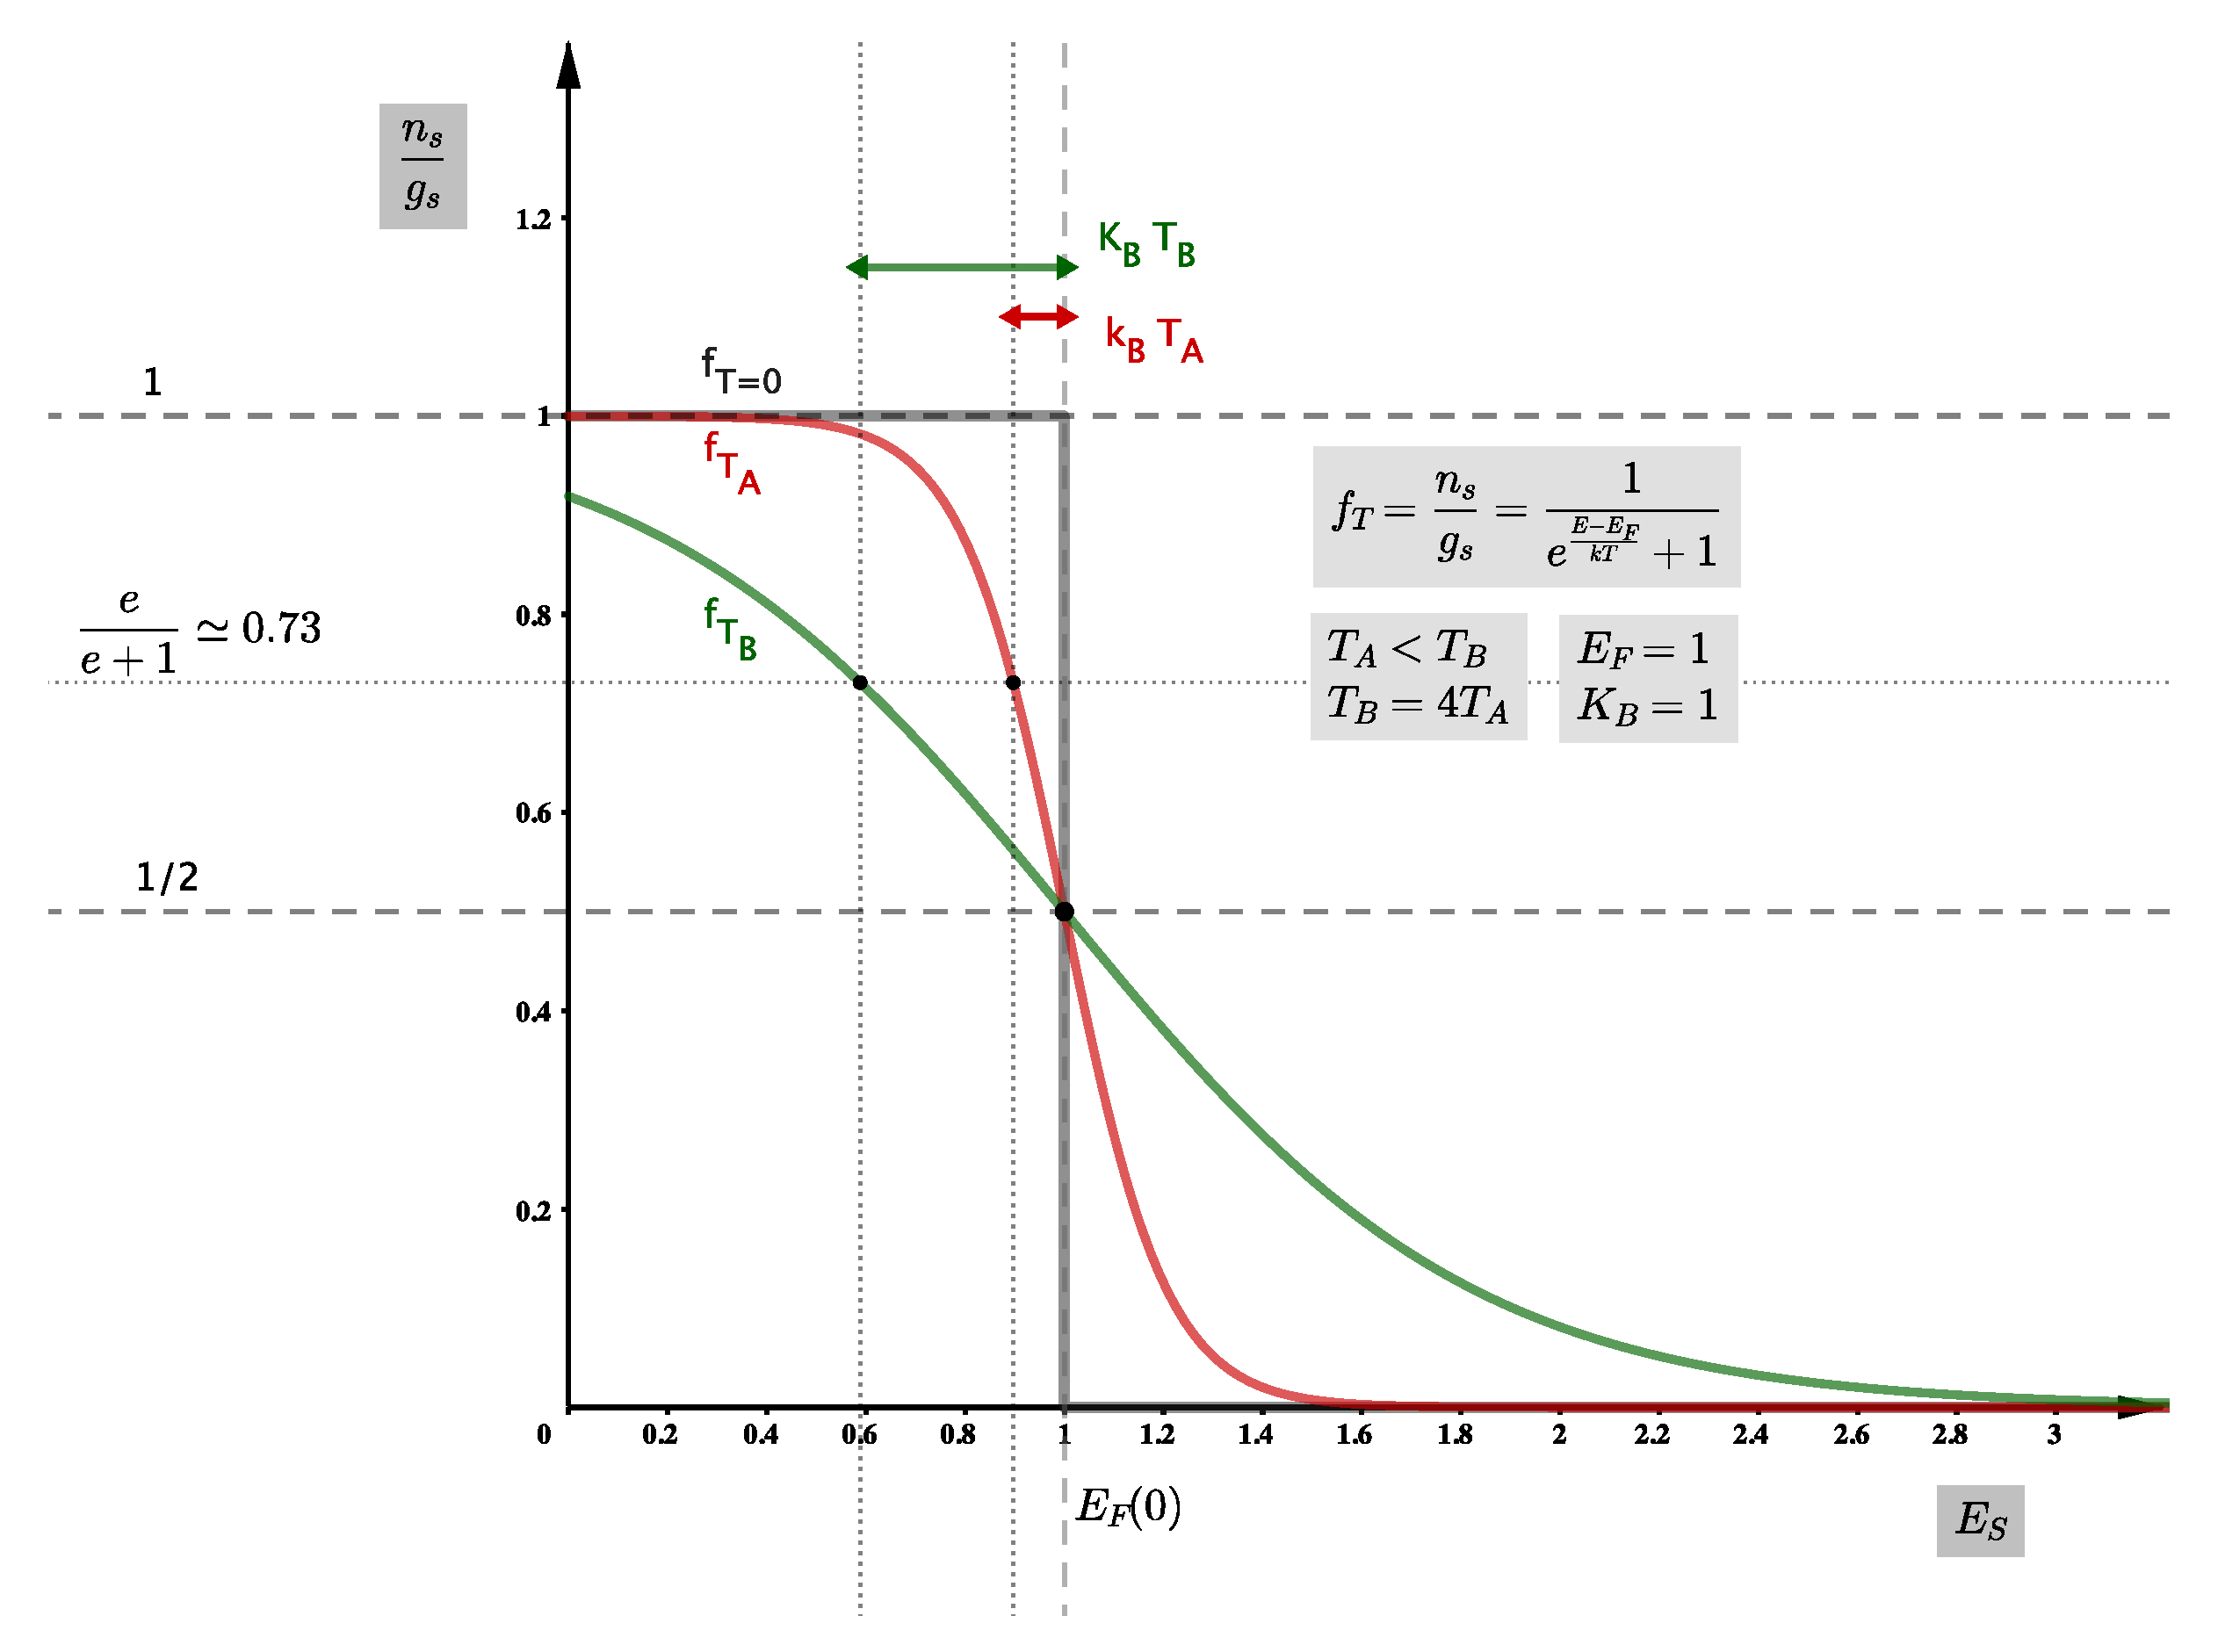
\includegraphics[scale=0.35]{/degenerazione3}
\label{grafico_distribuzioni}
\caption{Nel grafico vengono riportate tre distribuzioni calcolate su tre temperature, nel testo: \quad
Caso a) funzione $f_{T_A}$
Caso b) funzione $f_{T_B}$
Caso c) funzione $f_{T=\SI{0}{K}}$
}
\end{figure}

\subsection{Gas di elettroni}

Gli elettroni sono fermioni, la loro statistica è perciò descritta dal modello di Fermi-Dirac, poiché si tratta di particelle soggette al principio di esclusione di Pauli.
Gli \textbf{elettroni di conduzione nei metalli} sono un sistema quantistico anche a temperature \textit{normali} e non vicine allo zero assoluto, le densità tipiche di questi elettroni sono dell'ordine di $\SI{e28}{elettroni/m^3}$.

Quindi consideriamo un gas di elettroni, che seguono la statistica di Fermi Dirac, poiché fermioni, e si ha che la legge di distribuzione continua è la seguente, in cui compare $g(E)$ la \textit{funzione densità degli stati} (vedi \ref{fun_den_stat})
\begin{equation}
n(E)dE = \frac{ g(E)}{e^{ \frac{ E - E_F}{k_B T } } + 1 }
\quad\quad\quad\quad
g(E) = \frac{4 \pi V (2m^3)^{ \frac{1}{2} }}{h^3} E^{ \frac{1}{2} }
\end{equation}
trattandosi di elettroni, che hanno $spin=1/2$, gli stati disponibili raddoppiano e moltiplico x2, ottenendo
\begin{equation}
\begin{split}
n(E)dE & = 2 \cdot \frac{4 \pi V (2m^3)^{\frac{1}{2}} }{h^3} E^{\frac{1}{2}} \frac{1}{e^{\frac{E - E_F}{k_B T}} + 1} \\
& = \frac{8 \pi V (2m^3)^{\frac{1}{2}} E^{\frac{1}{2}}}{h^3} \frac{1}{e^{\frac{E - E_F}{k_B T}} + 1}
\label{nede_elet}
\end{split}
\end{equation}

\paragraph{Cerco l'espressione generale del Livello di Fermi}
Calcolo il numero totale delle particelle nel sistema, integrando in $[0, \infty]$, vedi figura \ref{fig_integrali_a}
\begin{equation}
N = \int_0^{\infty} n(E)dE
\end{equation}
Se suppongo di essere alla temperatura dello \textit{zero assoluto} la temperatura è $T=\SI{0}{K}$ per cui la distribuzione è rappresentata dalla funzione a gradino ed allora ha senso calcolare l'integrale nell'intervallo $[0, E_F(0)]$ dove la distribuzione vale 1, oltre il valore $E_F(0)$ la distribuzione (il secondo fattore nella \ref{nede_elet}) vale 0.
Per una rappresentazione grafica vedi figura \ref{fig_integrali_b}.
Per cui equivale a calcolare il seguente integrale
\begin{equation}
\begin{split}
N & = \int_0^{E_F(0)} g(E)dE \\
& = \int_0^{E_F(0)} \frac{8 \pi V (2m^3)^{\frac{1}{2}} E^{\frac{1}{2}}}{h^3} dE \\
& = \frac{8 \pi V (2m^3)^{\frac{1}{2}}}{h^3} \int_0^{E_F(0)} E^{\frac{1}{2}} dE \\
& = \frac{16 \pi V (2m^3)^{\frac{1}{2}}}{3 h^3} E_F(0)^{\frac{3}{2}}
\label{num_parti_N}
\end{split}
\end{equation}
Da cui posso ricavare un'espressione per il \textit{Livello di Fermi}
\begin{equation}
\begin{split}
E_F(0) & = \frac{h^2}{8m}\Bigl(  \frac{3N}{\pi V}  \Bigr)^{ \frac{2}{3} } \\
& = \frac{h^2}{8m}\Bigl(  \frac{3}{\pi} n  \Bigr)^{ \frac{2}{3} } \\
& = \frac{h^2}{8m}\Bigl(  \frac{3}{\pi}  \Bigr)^{ \frac{2}{3} } n^{ \frac{2}{3} }
\end{split}
\end{equation}
in cui $n=\frac{N}{V}$ è una densità, infatti è definito come il numero di particelle sul volume, è importante notare che il Livello di Fermi dipende da $n^{ \frac{2}{3} }$ e quindi cresce al crescere della densità.

\paragraph{Calcolo dell'energia totale del sistema}
È dato dall'integrale della funzione energia $E$ moltiplicata la distribuzione $n(E)$
\begin{equation}
U = \int_0^{\infty} E n(E) dE
\end{equation}
in cui è possibile utilizzare lo stesso ragionamento usato sopra ed integrare nell'intervallo $[0,E_F(0)]$
\begin{equation}
\begin{split}
U & = \int_0^{E_F(0)} E g(E) dE = \frac{8\pi V (2m^3)^{ \frac{1}{2} }}{h^3} \int_0^{E_F(0)} E^{ \frac{3}{2} } dE \\
& = \frac{2}{5} \frac{8\pi V (2m^3)^{ \frac{1}{2} }}{h^3} E_F(0)^{ \frac{5}{2} } = \frac{3}{5} N E_F(0)
\end{split}
\end{equation}
dove l'ultimo passaggio è possibile considerando il risultato ottenuto nella \ref{num_parti_N} per $N$. \\
L'\textbf{energia media per particella} è data da
\begin{equation}
\frac{U}{N} = \frac{3}{5} E_F(0)
\end{equation}
Questo risultato è importante in quanto ci dice che anche alla temperatura dello zero assoluto, quindi a $T = \SI{0}{K}$ l'energia media è diversa da zero, cosa che non succede classicamente in cui l'energia media è $U = n K T$ per cui a $T=\SI{0}{K}$ sarebbe nulla.

\paragraph{Pressione di Pauli} Per la termodinamica: la pressione che un gas esercita sulla parete è pari a
\begin{equation}
P = \frac{2}{3} \frac{U}{V}
\end{equation}
che per un gas di elettroni diventa
\begin{equation}
P = \frac{2}{3} \frac{U}{V} = \frac{2}{3V} \frac{3}{5} N E_F(0) = \frac{2}{5} n E_F(0) 
\end{equation}
detta \textit{Pressione di Pauli}.
Anche allo zero assoluto esiste una pressione \textit{residua} del sistema.

\begin{figure}[h]
    \centering
    \subfloat[In \textit{verde}: l'integrale ad una temperatura $T$ generica]{
        \label{fig_integrali_a}
        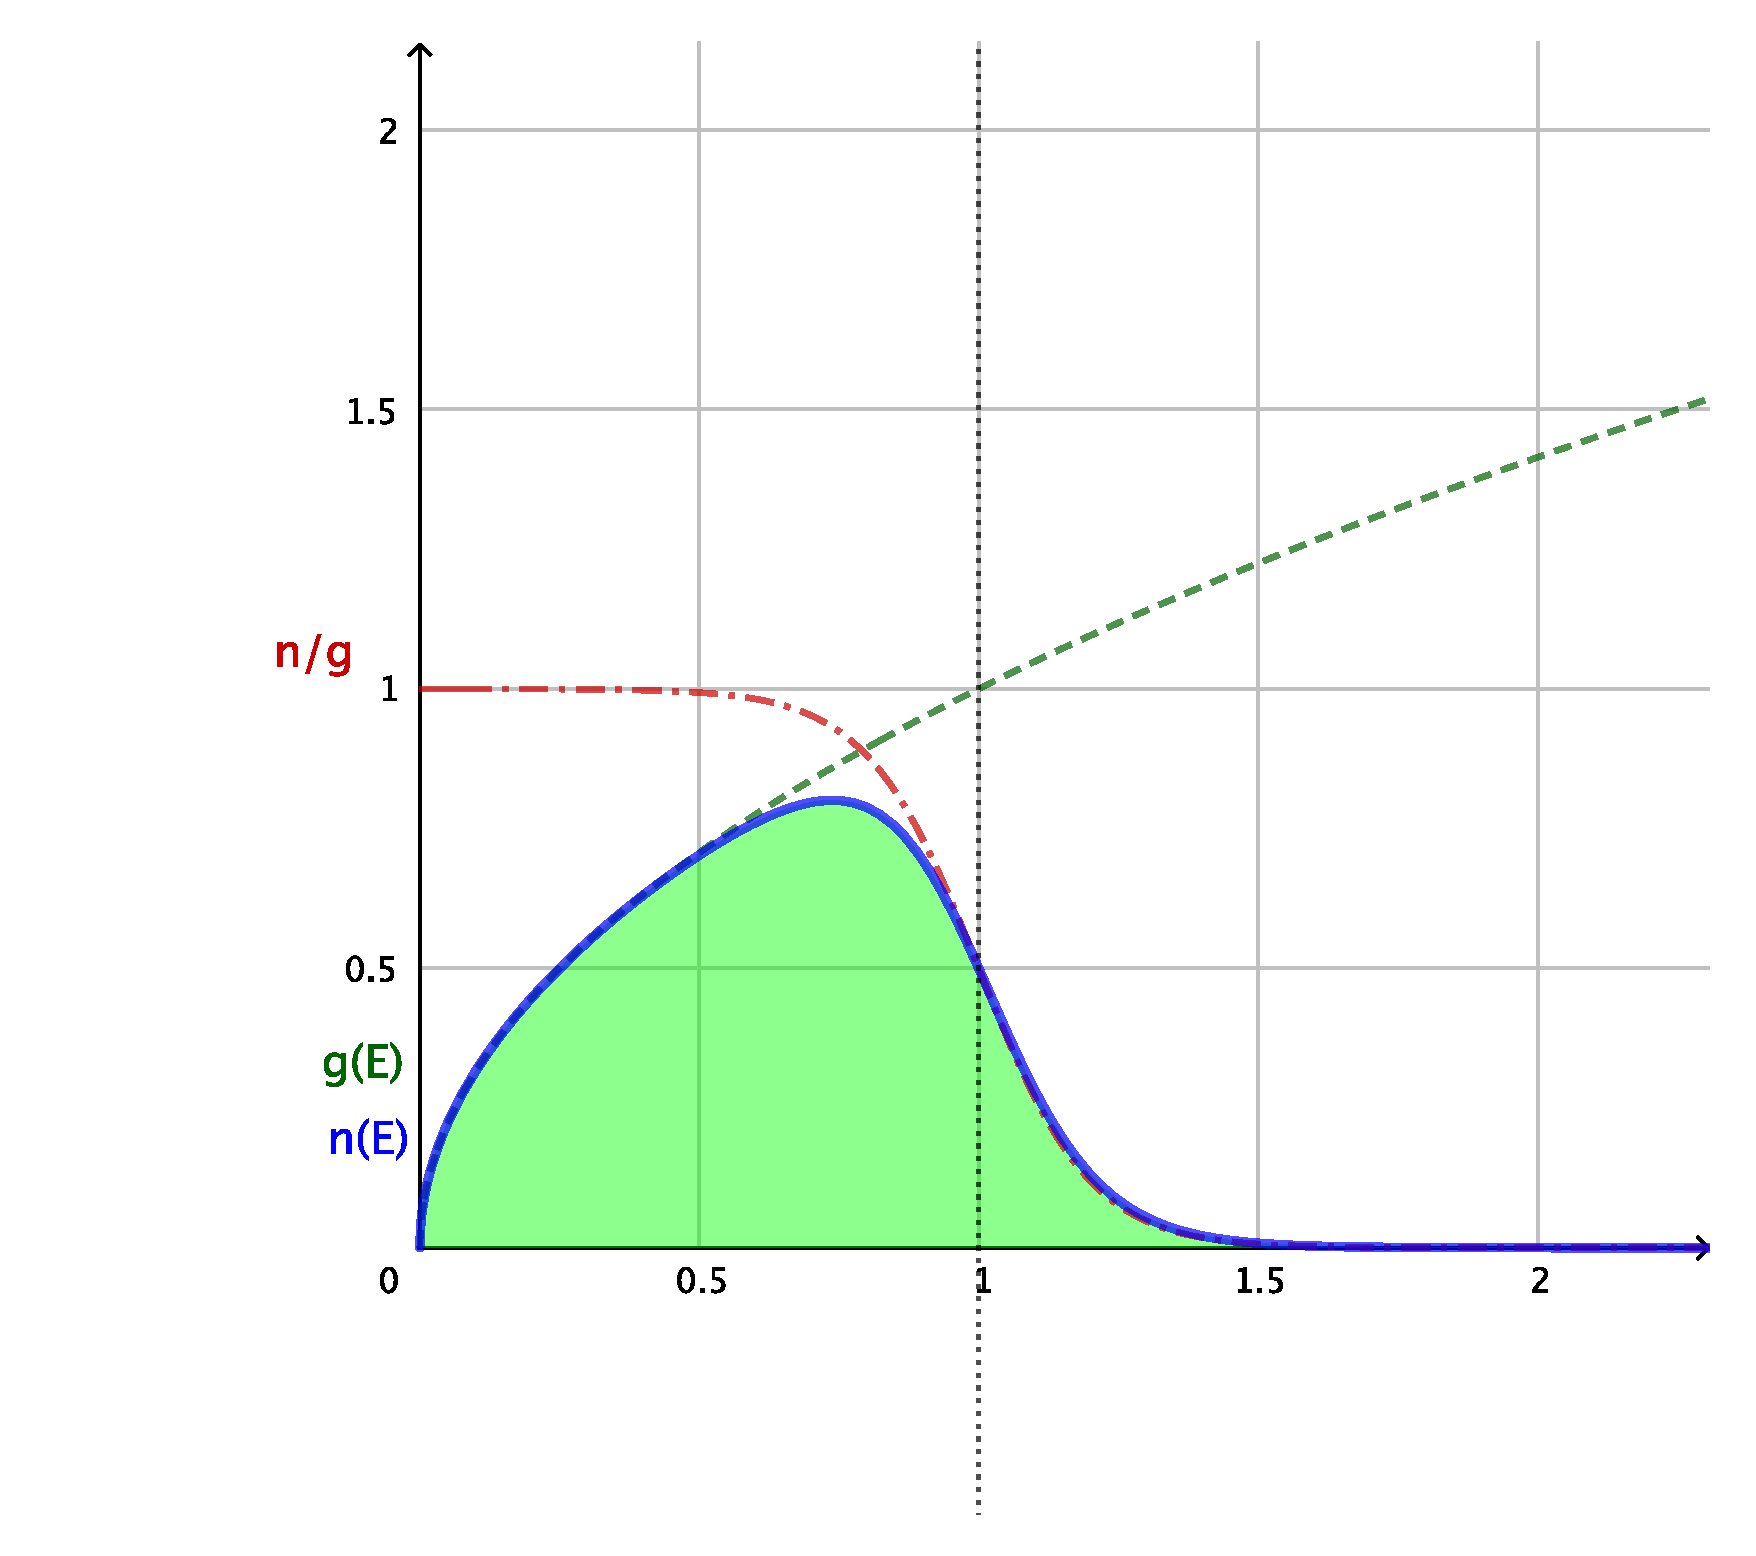
\includegraphics[ width=0.5\textwidth]{/integrale_1}
    }
    \subfloat[In \textit{blu}: l'integrale alla temperatura $T=\SI{0}{K}$]{
        \label{fig_integrali_b}
        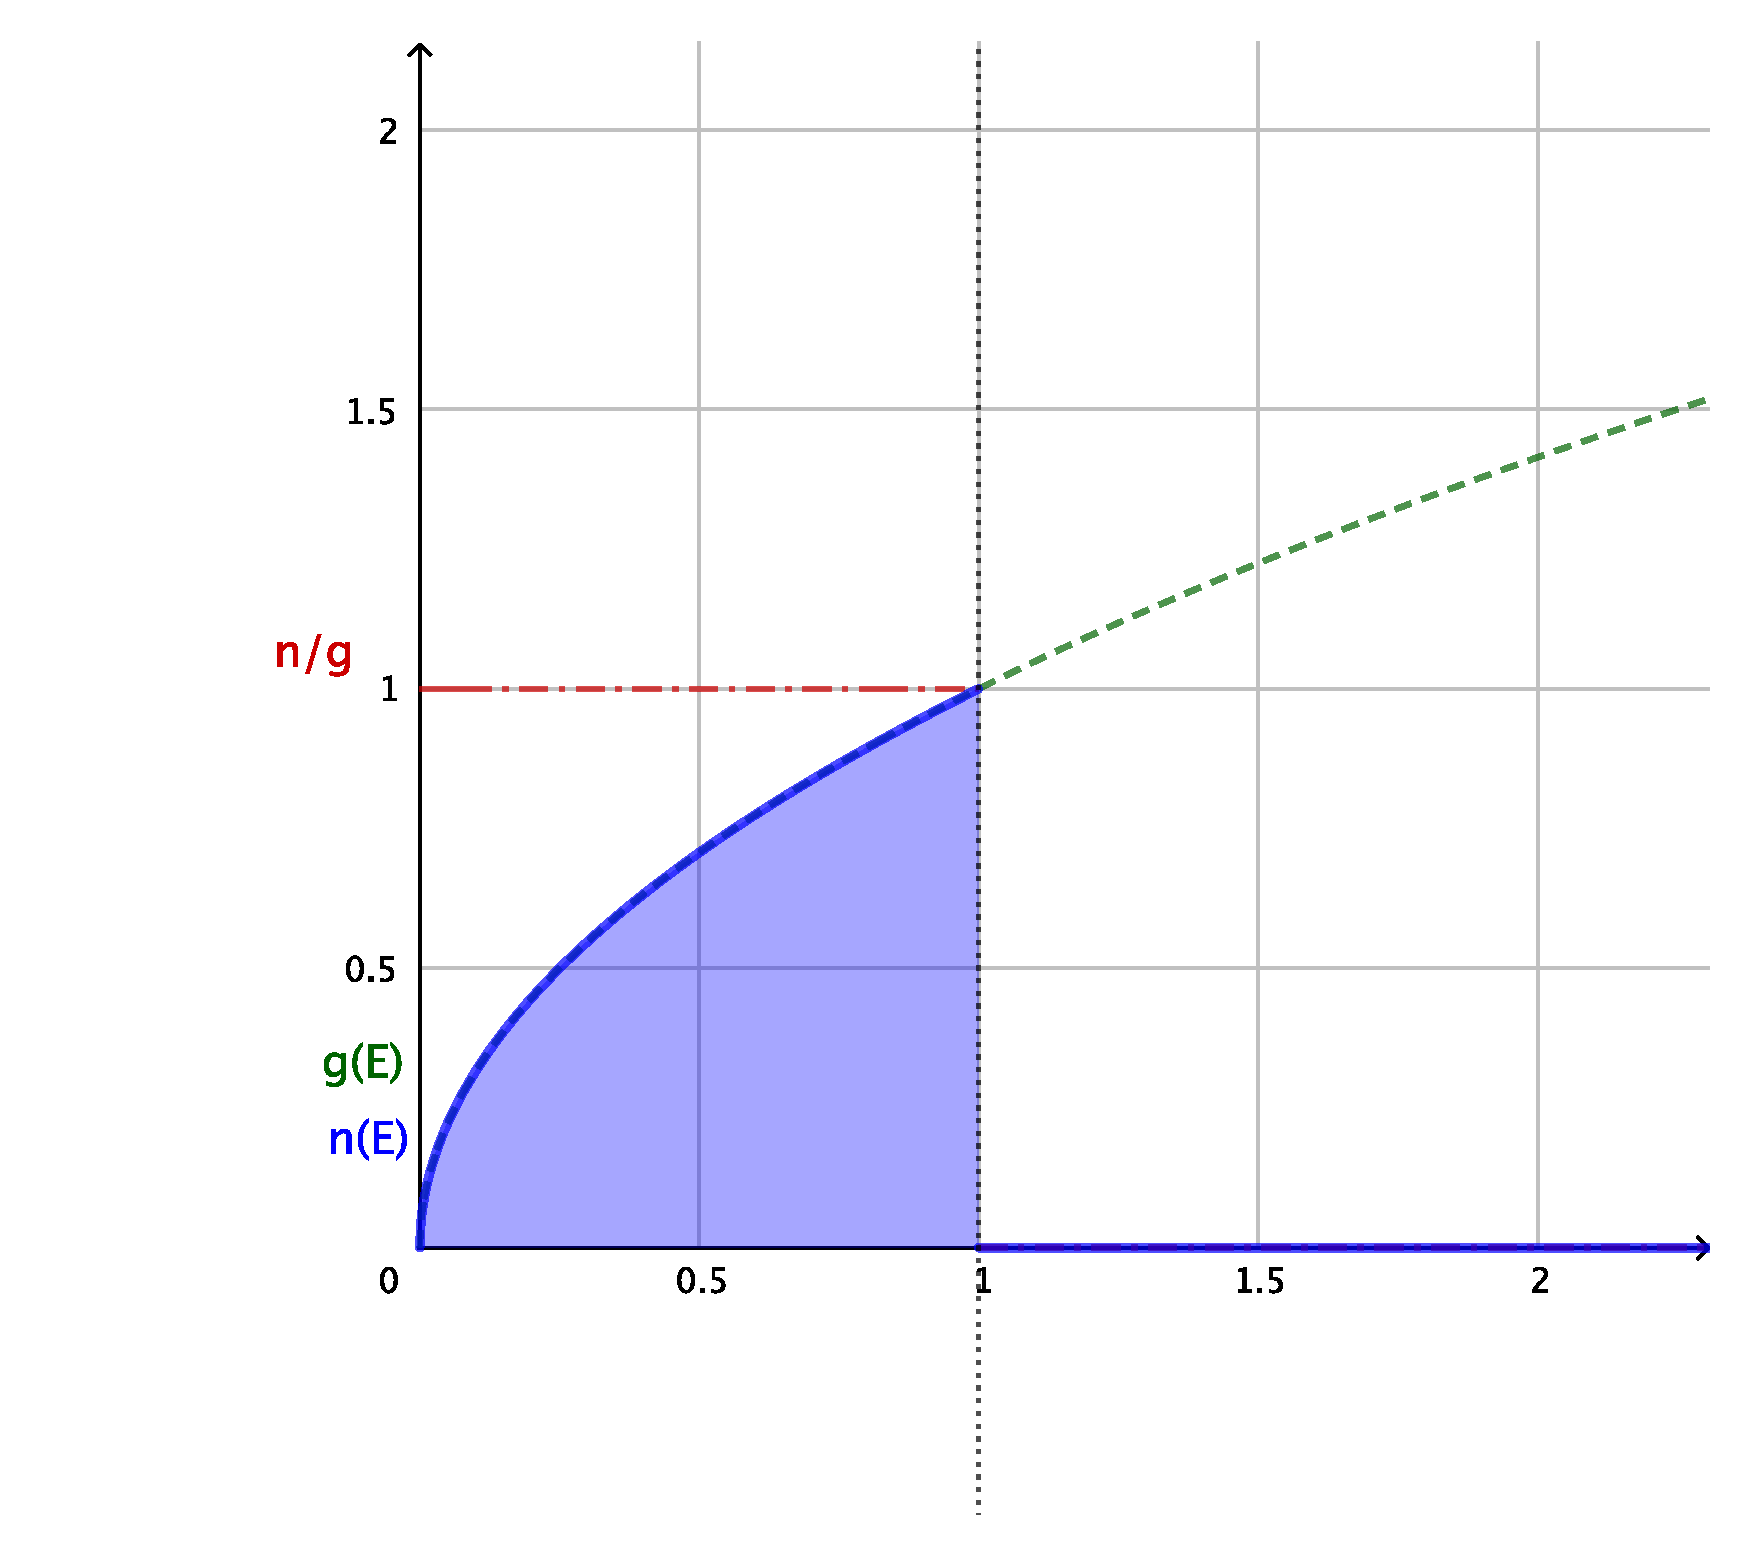
\includegraphics[ width=0.5\textwidth]{/integrale_2}
    }
    \caption{Gli integrali di questo capitolo vengono eseguiti a temperatura fissata $T=\SI{0}{K}$ per semplificare i conti, ciò è lecito poiché le due aree, \textit{verde} e \textit{blu} delle figure sopra, sono equivalenti.}
    \label{fig_integrali}
\end{figure}



\paragraph{Stima di $T_F$}
Nella teoria di Fermi Dirac, avendo fissato $\alpha$, ricavo il valore di $\xi$
\begin{equation}
\begin{split}
\alpha & = - \frac{E_F}{k_B T} \\
\xi & = e^{ -\alpha } = e^{ \frac{E_F}{k_B T} }
\end{split}
\end{equation}
se la temperatura è allo zero assoluto il parametro di degenerazione tende ad infinito per cui \textbf{il gas è totalmente degenere}
\begin{equation}
T=\SI{0}{K} \quad\Rightarrow\quad \xi \to + \infty
\end{equation}
le particelle sono "ammassate" nei livelli di più bassa energia, fino al Livello di Fermi.
Il gas rimane degenere fino a quando
\begin{equation}
k_B T \ll E_F(0) \quad\Rightarrow\quad T \ll T_F
\end{equation}
dove ribadiamo la Temperatura di Fermi \ref{temp_fermi}
$$T_F= \frac{E_F(0)}{k_B}$$
ovvero, per tali condizioni, si ha che l'Energia di Fermi $E_F$ coincide con il Livello di Fermi $E_F(0)$
\begin{equation}
\xi = e^{ \frac{E_F}{k_B T} } \simeq e^{ \frac{E_F(0)}{k_B T} } \gg 1
\end{equation}
Il gas non è degenere se
\begin{equation}
k_B T \gg E_F(0) \quad\Rightarrow\quad T \gg T_F
\end{equation}

Supponiamo un metallo in cui ogni atomo fornisce un elettrone alla banda di conduzione, quindi un metallo con \textit{valenza} 1 (numero di elettroni fornito da ogni atomo).
La distanza tra gli elettroni sia circa
\begin{equation}
d \simeq \SI{0.1}{n m} = \SI{1}{\AA}
\end{equation}
la densità
\begin{equation}
n = \frac{1}{d^3}
\end{equation}
stimiamo la Temperatura di Fermi
\begin{equation}
T_F = \frac{E_F(0)}{k_B} = \frac{h^2}{8k_B m} \Bigl(  \frac{3}{\pi}  \Bigr)^{ \frac{2}{3} } n^{ \frac{2}{3} }
\end{equation}
considero che 
\begin{equation}
n^{ \frac{2}{3} } = \Bigl(  \frac{1}{d^3}  \Bigr)^{ \frac{2}{3} } = d^{ -2 }
\end{equation}
allora la Temperatura di Fermi risulta
\begin{equation}
\begin{split}
T_F = 
\end{split}
\end{equation}





\newpage
\iffalse

Poiché $\alpha = -\frac{ E_F}{k T} \quad \Rightarrow \quad \xi = e^{-\alpha} = e^{ \frac{ E_F}{k T}}$ allora si ha che per $T=\SI{0}{K} \Rightarrow \xi = +\infty $
e si è in presenza di un gas totalmente degenere, che significa, nel caso di fermioni, che le particelle sono tutte "ammassate", pur rispettando il Principio di Esclusione di Pauli, nei livelli più bassi.
Un gas di fermioni continua a rimanere degenere se $T \ll T_F$ dove $T_F = \frac{ E_F(0)}{k}$, cioè se $kT \ll E_F(0)$, 
dove $E_F(T) \approx E_F(0)$ e quindi $\xi \gg 1$
In tal caso occorre usare la statistica di Fermi-Dirac.
Tuttavia se $kT \gg E_F(0) \Rightarrow T \gg T_F $, si deve (o si può?) applicare la statistica classica.

Supponiamo ora di avere un metallo di \underline{valenza 1} (la valenza esprime quanti elettroni di conduzione possono essere forniti da ogni atomo del metallo).
Supponiamo che la distanza fra gli elettroni sia $a \simeq \SI{0.1}{nm}$, allora una stima della densità elettronica è $n = \frac{ 1}{a^{ 3}} = a^{ -3}$.
Stimiamo $T_F$, perciò:

\begin{equation}
\begin{cases}
	T_F = \frac{ E_F(0)}{k} = \frac{ h^2}{8 k m} \Bigl(  \frac{ 3}{\pi}  \Bigr)^{ \frac{ 2}{3}} n^{ \frac{ 2}{3}} \simeq \frac{ h^2}{k m a^2} \simeq \frac{ 10^{ -68}}{10^{-23 } 10^{ 30} 10^{-20 }} \frac{ J \cdot s^2 \cdot K}{J \cdot Kg \cdot m^2} = 10^{5} K \\
	n^{ \frac{ 2}{3}} = \Bigl(  a^{ -3}  \Bigr)^{ \frac{ 2}{3}} = a^{ -2}
\end{cases}
\end{equation}

$T_F$ separa il regime di Fermi-Dirac da quello classico di Maxwell-Boltzmann, ed essendo dell'ordine di $10^{ -5}$, si ha che in situazioni ordinarie il sistema di elettroni è sempre degenere.
Il calcolo precedente è semplice perché si ha a che fare con lo zero assoluto, mentre le cose si complicano per $T \not =\SI{0}{K} $.

Studiamo ora la \underline{capacità termica} $C_V$, a volume costante: tale grandezza è legata a $T$ (temperatura assoluta).
Il contributo fondamentale alla capacità termica è dato dal reticolo del solido cristallino, ora studiamo il contributo elettronico.
Solo una frazione delle particelle vede variare la propria energia, perché siamo nel caso $T \not = o \ll T_F$, e tale variazione è:
$$ \Delta U \simeq N \frac{ k T}{E_F(0)} kT \simeq N\Bigl(  \frac{ T}{T_F}  \Bigr)kT $$

Poiché $C_V = \frac{ dU}{dT} \simeq N k \Bigl(  \frac{ T}{T_F}  \Bigr) $ usando $U = \frac{ 3}{2} N k T$ si ha che $C_V = \frac{ 3}{2} N k$ 
ed è allora necessario che $T$ sia confrontabile con $T_F \quad (T \approx T_F)$, ma ciò non accade nel caso ordinario per i fermioni,
per i quali quindi $C_V = C_V(T)$, e in particolare:
\begin{equation}
C_V = \frac{ \pi^2}{2} N k \Bigl(  \frac{ T}{T_F}  \Bigr)
\end{equation}

\begin{figure}[h]
\centering
\includegraphics[scale=0.1]{/buca_potenziale}
\caption{Buca di potenziale in un metallo}
\end{figure}

Consideriamo ora una \underline{buca di potenziale}: \\

Funzione lavoro $W_0 = h\nu_0 \Rightarrow V_0 = E_F(0) + W_0$ ed in generale si ha che $V_0$ è dell'ordine di qualche $eV$,
ad esempio l'argento ha $W_0 = \SI{4.7}{eV}$ e $ E_F(0) = \SI{5.5}{eV} $
Gli elettroni nel metallo riempiono i livelli energetici fino a $E_f(0)$. 
$W_0$ nei metalli è generalmente tale che $\SI{5}{eV} < V_0 < \SI{15}{eV} $

Questo spiega l'\underline{effetto termoionico}: è un fenomeno per cui un metallo riscaldato ad una temperatura sufficientemente alta inizia ad emettere elettroni presenti sulla sua superficie. A $T \noT=\SI{0}{K} $ gli elettroni cominciano ad occupare gli strati più elevati e ad uscire dalla buca di potenziale.

\fi














